\documentclass{article}
\usepackage[utf8]{inputenc}
\usepackage[shortlabels]{enumitem}
\usepackage{geometry}
\geometry{a4paper,left=20mm,right=20mm, top=10mm}
\usepackage{graphicx}
\usepackage{float}
\usepackage{amsmath}
\usepackage{bm}
\usepackage{dsfont}
\usepackage{upgreek}
\usepackage{float}
\usepackage{subcaption}
\usepackage{graphicx} 
\usepackage{hyperref}
\usepackage{tikz}
\usetikzlibrary{arrows}
\usepackage{array}
\setlength\parindent{0pt}
\begin{document}

1.	Generate synthetic data directly from probabilistic model. I have tried different kernels, such as non-linear over inputs + non-linear over outputs, or + linear over outputs. Both GPAR and GPLAR can fit to those data. GPLAR performs better when a). there is large noise in the observations, b). different noise level in different outputs.

\begin{figure}[H]
\centering
\includegraphics[width=.8\linewidth]{noise-01.png}
\caption{SE kernel over inputs + SE kernel over outputs + noise variance=0.1}
\end{figure}

\begin{figure}[H]
\centering
\includegraphics[width=.8\linewidth]{noise-05.png}
\caption{SE kernel over inputs + SE kernel over outputs + noise variance=0.5}
\end{figure}

\begin{figure}[H]
\centering
\includegraphics[width=.8\linewidth]{noise-different.png}
\caption{SE kernel over inputs + SE kernel over outputs + different noise level for every output}
\end{figure}


\begin{figure}[H]
\centering
\includegraphics[width=.8\linewidth]{Linear-output.png}
\caption{SE kernel (with different length-scales) every output over inputs + Linear kernel over outputs + noise variance = 0.1}
\end{figure}

\newpage
2.	I have looked into weird behavior of GPAR over the synthetic third output last time in the log-density vs observation noise, such that log-density of the third output can be extremely high sometimes. I have made a mistake that I didn’t calculate the log-density over held-out datasets, but over training datasets and GPAR can sometimes overfit as shown below. 
\begin{figure}[H]
\centering
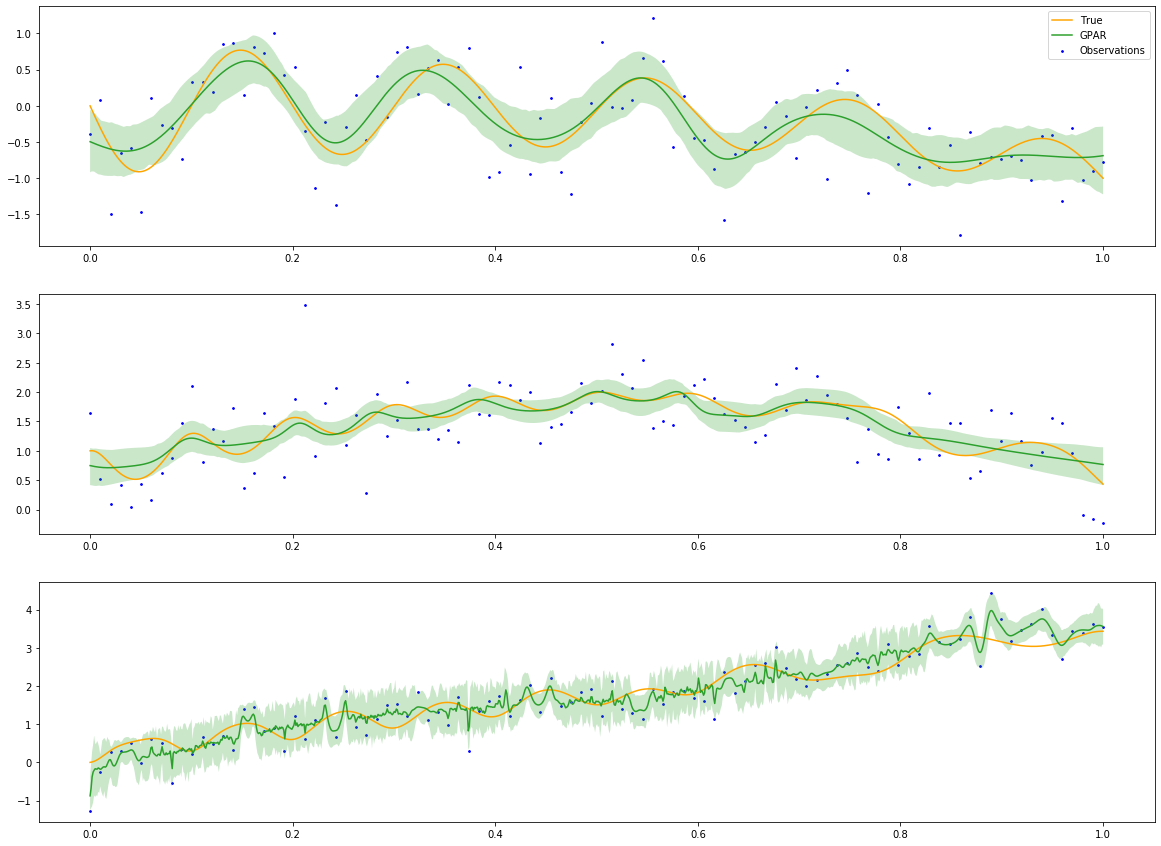
\includegraphics[width=.8\linewidth]{gpar-run-3.png}
\caption{Third output overfits severely, making the log-density very high}
\end{figure}
\begin{figure}[H]
\centering
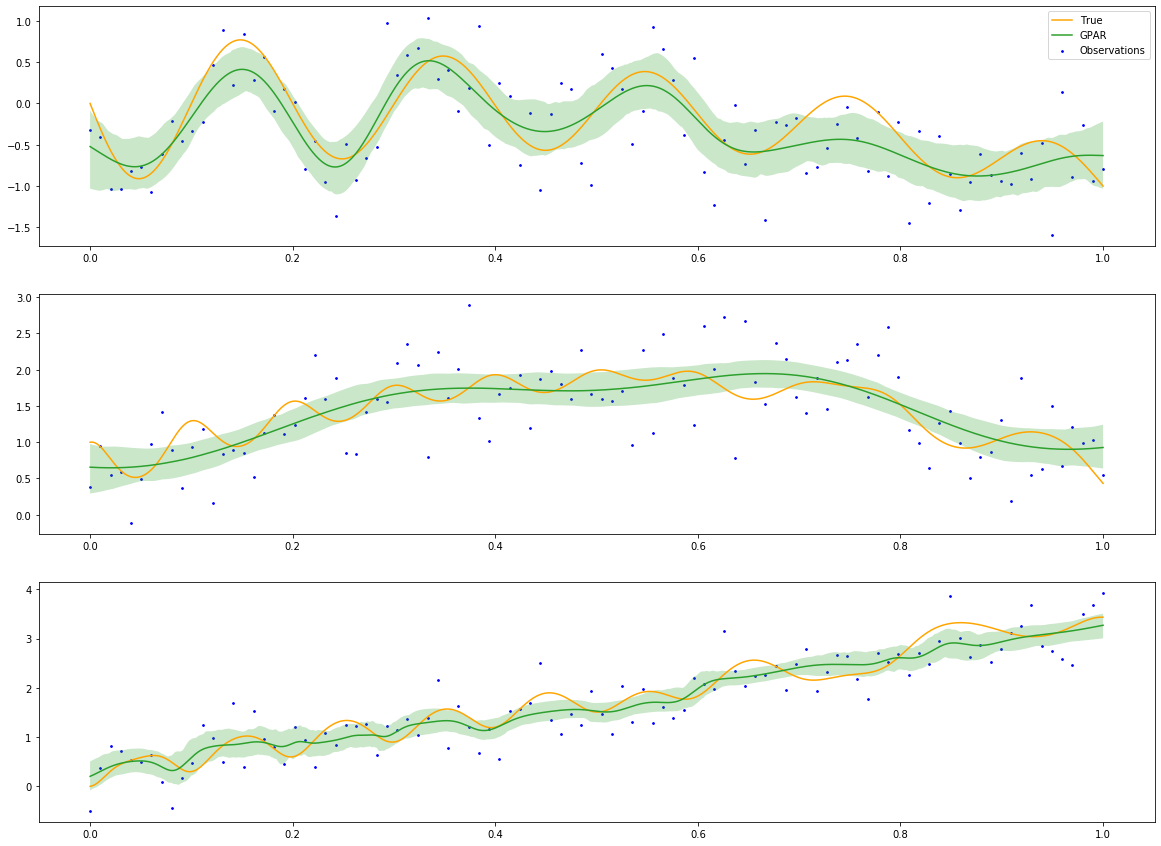
\includegraphics[width=.8\linewidth]{gpar-run-4.png}
\caption{Sometimes, third output underfits severely, hence log-density’s variance is high}
\end{figure}

Instead, I run the held-out log-likelihood vs noise using the synthetic data generated from first task. And this time log-likelihood is calculated over test dataset never observed during training. 100 trials of different noise seed are run and np.percentile are used to produce 2.5-97.5\% bounds.

\begin{figure}[H]
\centering
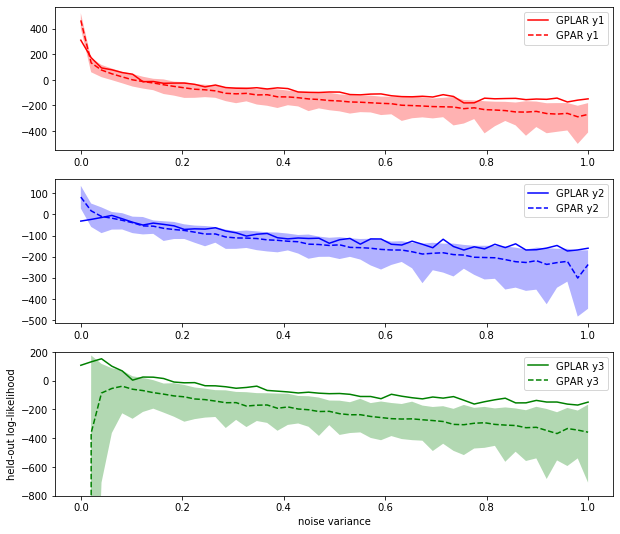
\includegraphics[width=.8\linewidth]{hll.png}
\caption{hll-vs-noise}
\end{figure}

Again, the third output held-out loglikelihoods for GPAR are weird when noise variance is close to zero. I checked why, and it turned out that GPAR’s predictive variance for third output are all near zero, (1e-7 level), making the log-likelihood extremely negative if the true value is slightly away from the predictive mean. But GPLAR’s predictive variance is at an appropriate level. It is observed that GPLAR’s held-out log-likelihood is always overlap or better than GPAR’s upper bounds. I can also run GPLAR for more runs of seeds, but it will require more time.
\newpage
3.	To make GPLAR work in close-upwards observations. \\
a)	I have tried i). completely remove temporal kernels, ii). using additive kernels over outputs. Both methods cannot work. \\
b)	I also sanity check that when q\_mu is initialized over missing areas using the true observations, “q\_mu” would not run away from them during optimization. \\
c)	Hence, I implemented the bi-directional version of GPLAR, such that a DGP run in reverse is added. And the model can produce good results as shown below, without losing its good performance on close-downwards observations. (I first initialized q\_mu to be the corresponding output posterior mean of GPAR, but it trained rather slowly, and then I realized in normal DGP, all q\_mu is initialized to zero, which will train much faster with similar time as when reverse DGP are not added. Waste some time on realizing this).

\begin{figure}[H]
\centering
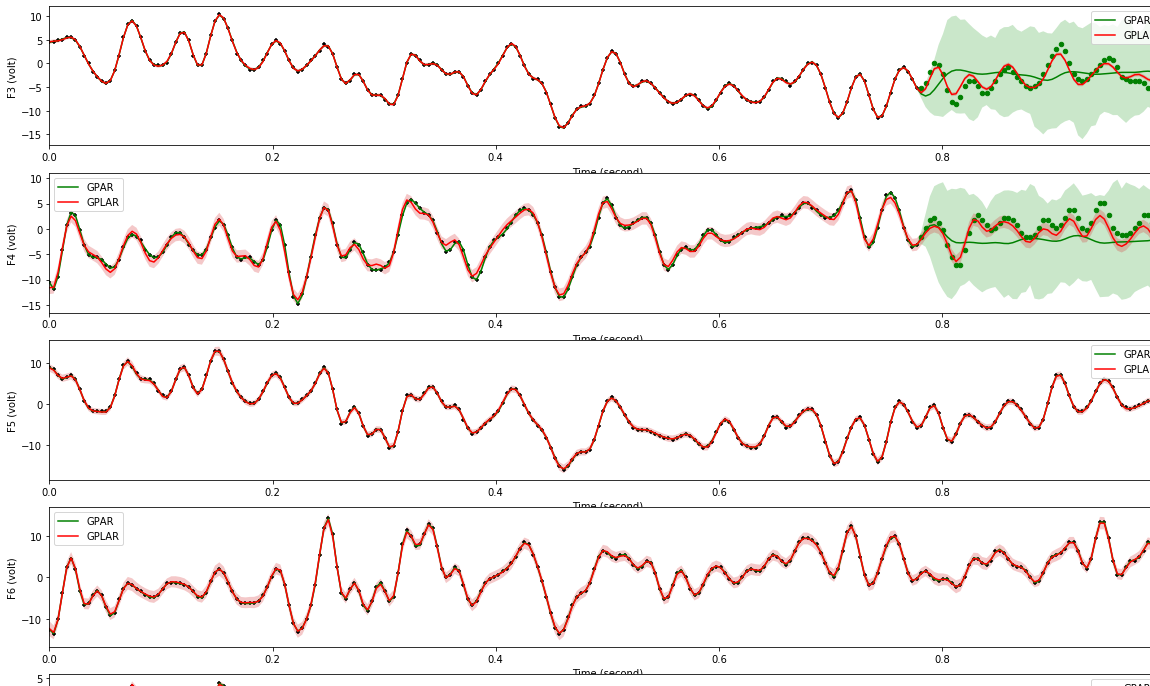
\includegraphics[width=.8\linewidth]{eeg-bidirectional-1-.png}
\caption{Only 50 missing datapoints in first two outputs (last 4 outputs are cropped)}
\end{figure}

\begin{figure}[H]
\centering
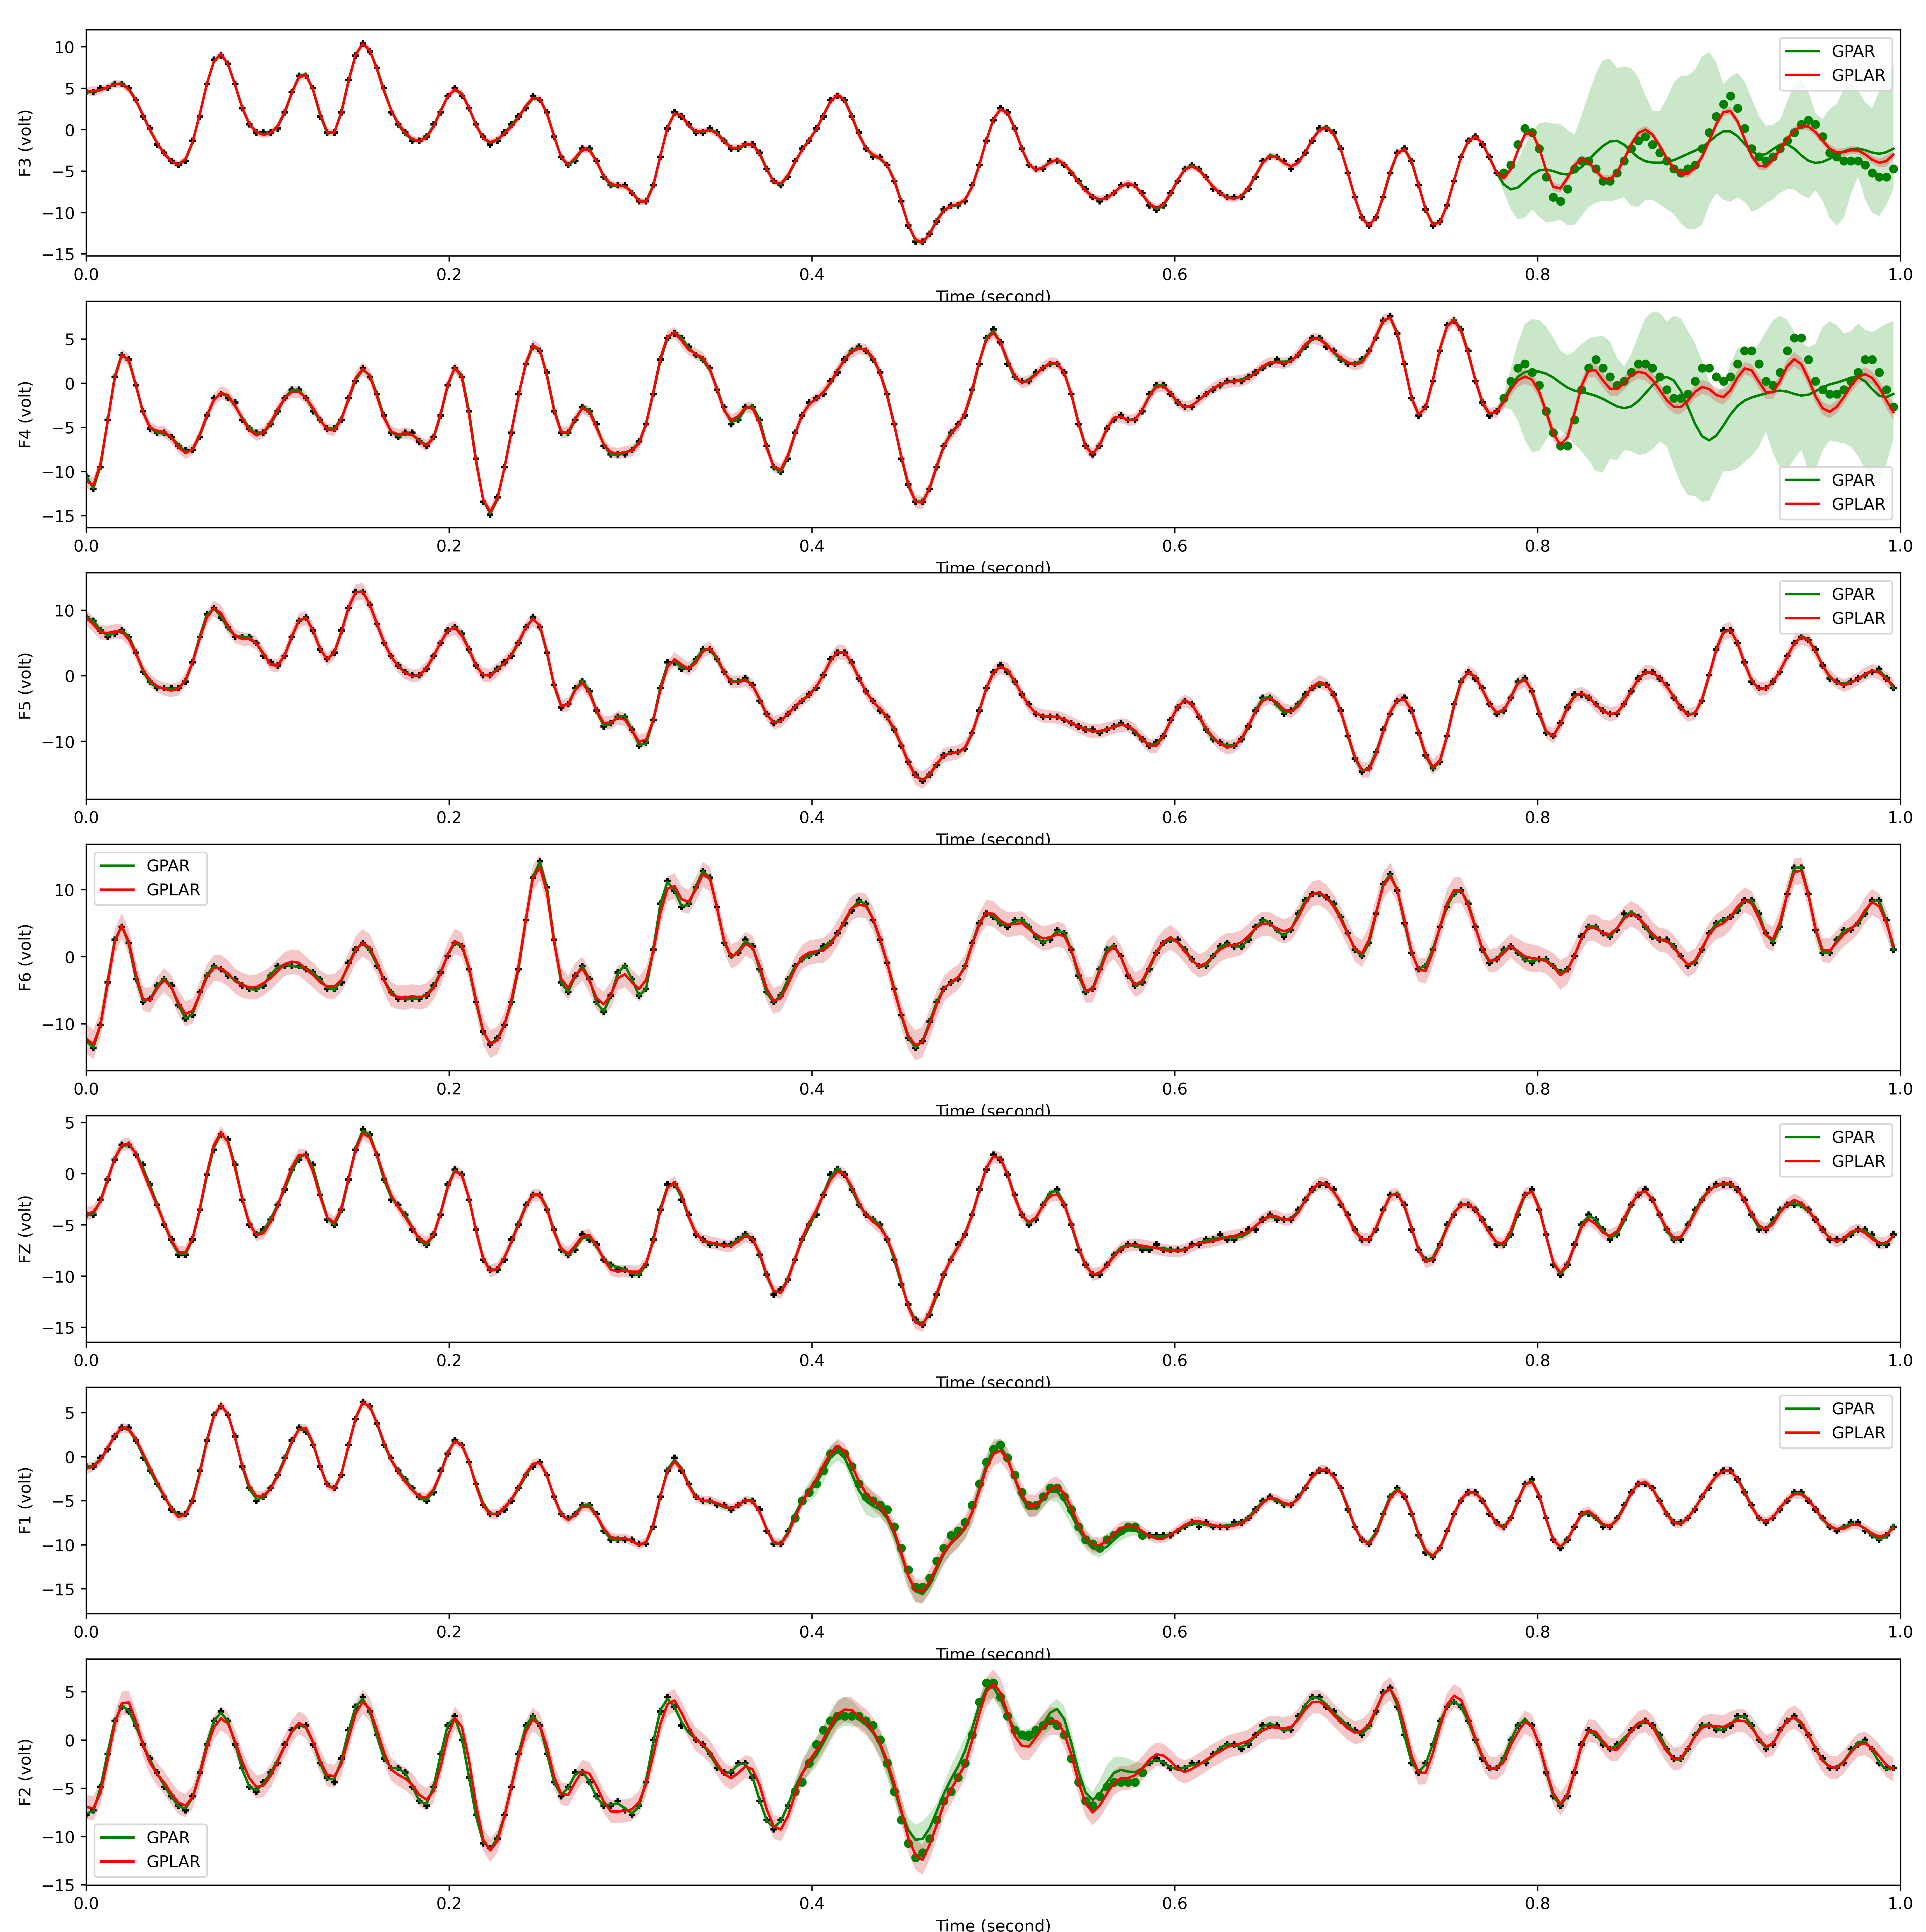
\includegraphics[width=.8\linewidth]{eeg-bidirectional-2.png}
\caption{50 missing datapoints in first two outputs (0.8-1.0) are last two outputs (0.4-0.6)}
\end{figure}

\begin{figure}[H]
\centering
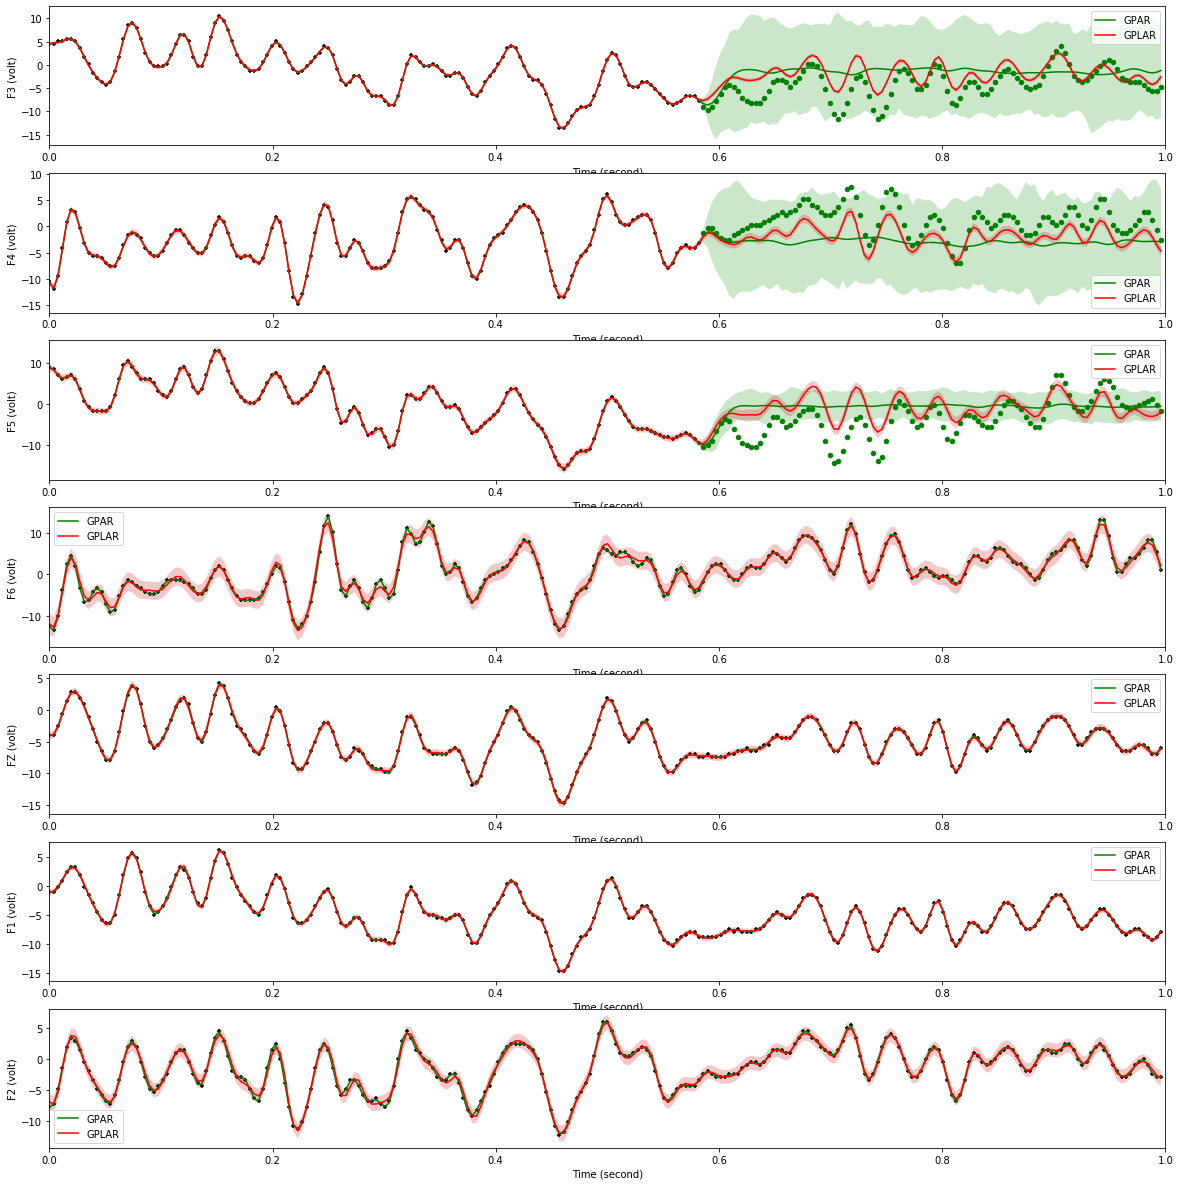
\includegraphics[width=.8\linewidth]{eeg-bidirectional-3.png}
\caption{However, GPLAR can performed badly both on bias and variance when missing area is large and there are more outputs with missing area. Will the simple normalization strategy be a problem here?}
\end{figure}

Exchange-rate dataset is always harder to fit as compared to EEG dataset. Nevertheless, bi-direction version GPLAR performs better than normal version. 

\begin{figure}[H]
\centering
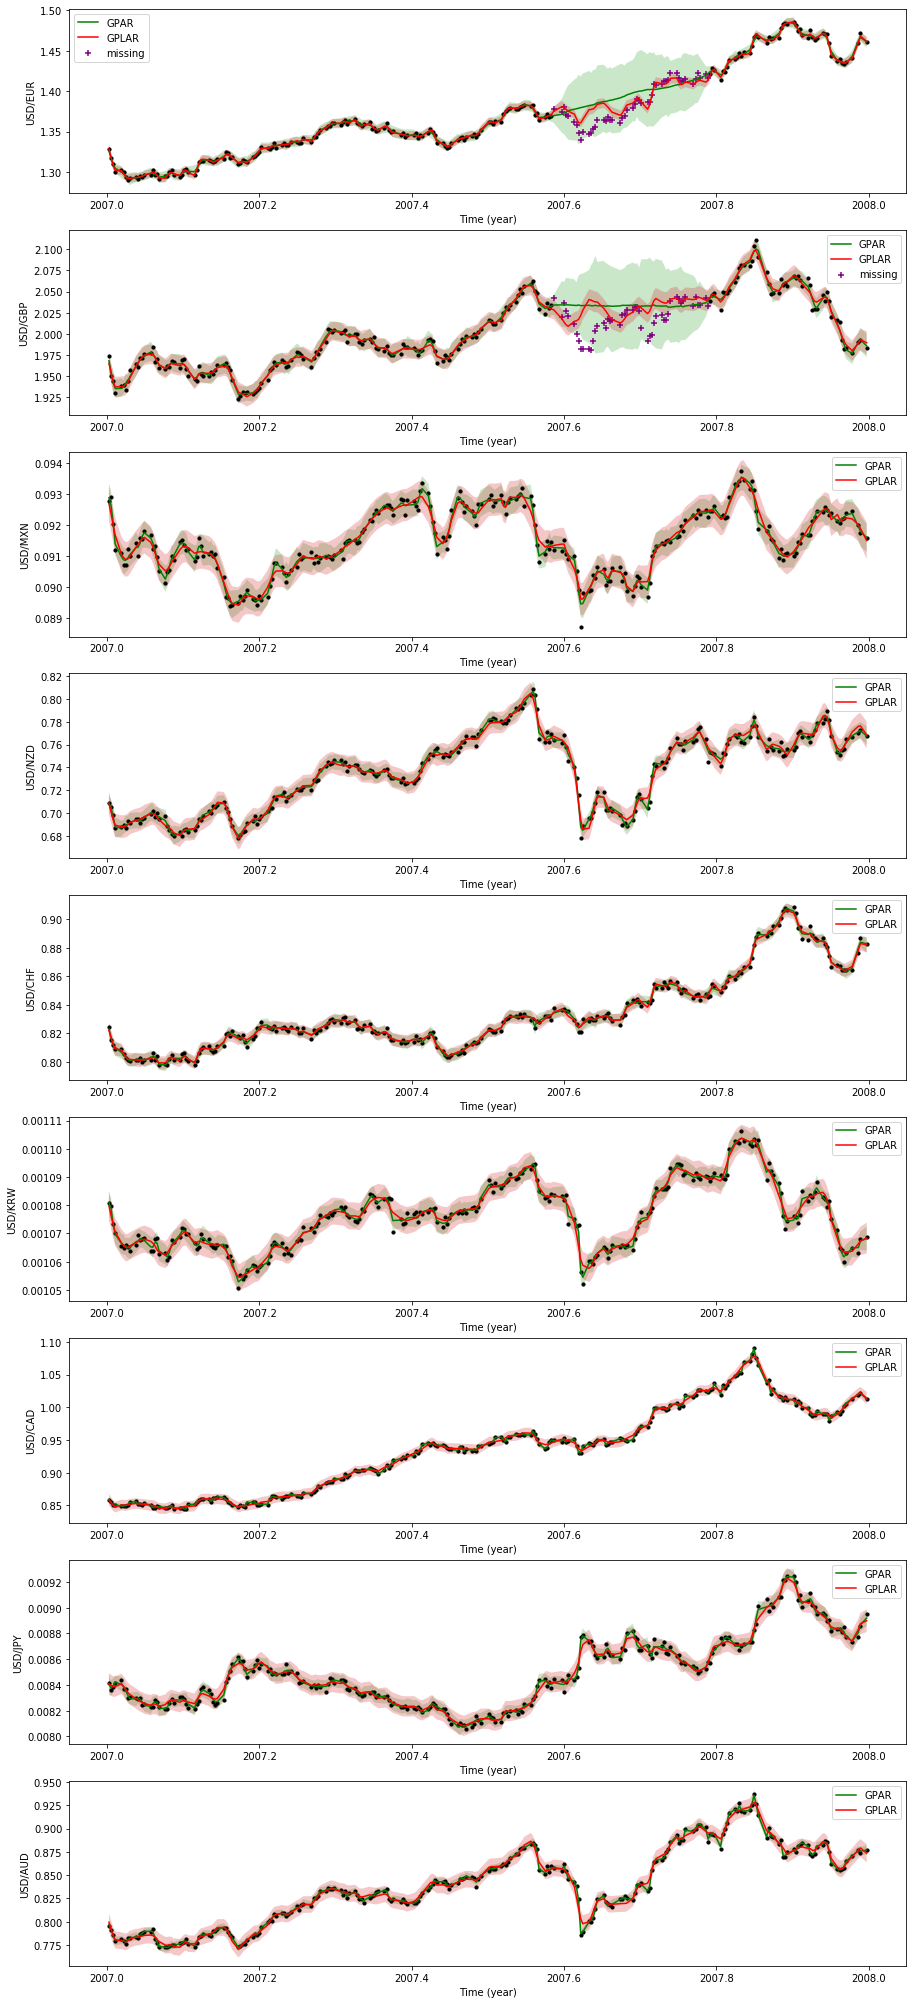
\includegraphics[width=.6\linewidth]{exchange-bidirectional-2.png}
\end{figure}


\begin{figure}[H]
\centering
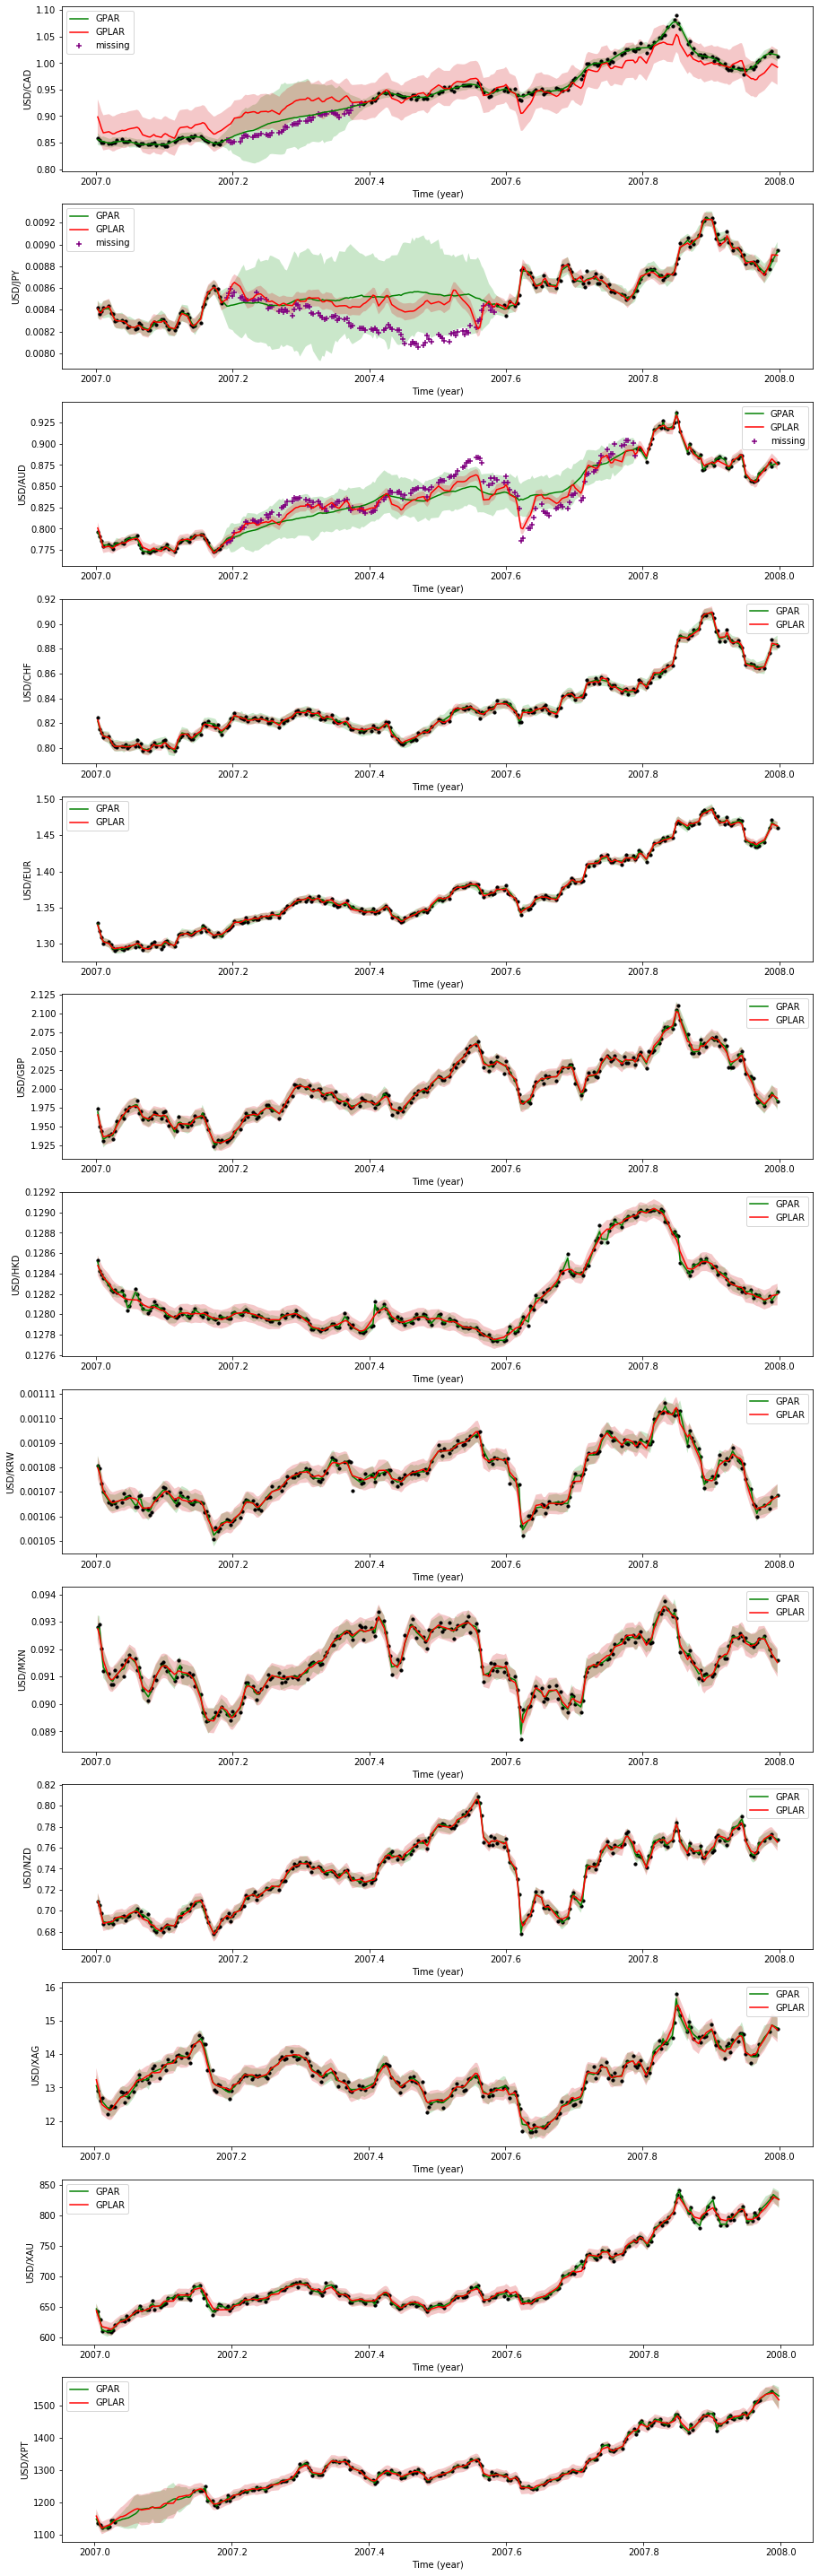
\includegraphics[width=.6\linewidth]{exchange-bidirectional-3.png}
\end{figure}

\end{document}
